\documentclass[12pt,a4paper]{report}

\usepackage[T1]{fontenc}
\usepackage[utf8]{inputenc}
\usepackage[italian]{babel}
\usepackage{bold-extra}
\usepackage{tocloft}
\usepackage{titlesec}
\usepackage{float}
\usepackage{amsmath}
\usepackage{hyperref}
\usepackage{graphicx}
\usepackage{listings}
\usepackage{minted}

% !TeX root = main.tex

\textwidth=450pt
\oddsidemargin=0pt

\setcounter{tocdepth}{3}
\setcounter{secnumdepth}{3}

\renewcommand{\cftpartleader}{\cftdotfill{\cftdotsep}} % for parts
\renewcommand{\cftchapleader}{\cftdotfill{\cftdotsep}} % for chapters

\titleformat{\chapter}{\Huge\bfseries}{\chaptername\ \thechapter}{0pt}{\vskip 100pt\raggedright}%
% Alter <after-sep> in the macro below to vary the separation after the \chapter title.
\titlespacing{\chapter}{0pt}{50pt}{50pt}
% \titlespacing{<command>}{<left>}{<before-sep>}{<after-sep>}[<right>]

% configura i lettori pdf
\hypersetup{%
  pdfpagemode={UseNone},
  hidelinks,                  % nasconde i collegamenti (non vengono quadrettati)
  hypertexnames=false,
  linktoc=all,                % inserisce i link nell'indice
  unicode=true,               % usa solo caratteri Latini nei segnalibri di Acrobat
  pdftoolbar=false,           % nasconde la toolbar di Acrobat
  pdfmenubar=false,           % nasconde il menu di Acrobat
  plainpages=false,
  breaklinks,
  pdfstartview={Fit},
  pdflang={it}
}

\lstdefinelanguage{Kotlin}{
  comment=[l]{//},
  commentstyle={\color{gray}\ttfamily},
  emph={filter, first, firstOrNull, forEach, lazy, map, mapNotNull, println},
  emphstyle={\color{OrangeRed}},
  identifierstyle=\color{black},
  keywords={!in, !is, abstract, actual, annotation, as, as?, break, by, catch, class, companion, const, constructor, continue, crossinline, data, delegate, do, dynamic, else, enum, expect, external, false, field, file, final, finally, for, fun, get, if, import, in, infix, init, inline, inner, interface, internal, is, lateinit, noinline, null, object, open, operator, out, override, package, param, private, property, protected, public, receiveris, reified, return, return@, sealed, set, setparam, super, suspend, tailrec, this, throw, true, try, typealias, typeof, val, var, vararg, when, where, while},
  keywordstyle={\color{NavyBlue}\bfseries},
  morecomment=[s]{/*}{*/},
  morestring=[b]",
  morestring=[s]{"""*}{*"""},
  ndkeywords={@Deprecated, @JvmField, @JvmName, @JvmOverloads, @JvmStatic, @JvmSynthetic, Array, Byte, Double, Float, Int, Integer, Iterable, Long, Runnable, Short, String, Any, Unit, Nothing},
  ndkeywordstyle={\color{BurntOrange}\bfseries},
  sensitive=true,
  stringstyle={\color{ForestGreen}\ttfamily},
}

\setminted[terraform]{
  linenos=true,
  breaklines=true,
  encoding=utf8,
  fontsize=\footnotesize,
  frame=lines
}

\setminted[java]{
  linenos=true,
  breaklines=true,
  encoding=utf8,
  fontsize=\footnotesize,
  frame=lines
}

\setminted[docker]{
  linenos=true,
  breaklines=true,
  encoding=utf8,
  fontsize=\footnotesize,
  frame=lines
}

\setminted[yaml]{
  linenos=true,
  breaklines=true,
  autogobble,
  encoding=utf8,
  fontsize=\footnotesize,
  frame=lines
}

\setminted[bash]{
  linenos=true,
  breaklines=true,
  autogobble,
  encoding=utf8,
  fontsize=\footnotesize,
  frame=lines
}

\setminted[toml]{
  linenos=true,
  breaklines=true,
  autogobble,
  encoding=utf8,
  fontsize=\footnotesize,
  frame=lines
}

\setminted[kotlin]{
  linenos=true,
  breaklines=true,
  autogobble,
  encoding=utf8,
  fontsize=\footnotesize,
  frame=lines
}

\setminted[ruby]{
  linenos=true,
  breaklines=true,
  encoding=utf8,
  fontsize=\footnotesize,
  frame=lines
}

\begin{document}
  
\begin{titlepage}
\begin{center}
{{\Large{\textsc{Alma Mater Studiorum $\cdot$ Universit\`a di
Bologna\\\vspace{2mm}Campus di Cesena}}}} \rule[0.1cm]{15.8cm}{0.2mm}

{\small{\textsc { DIPARTIMENTO DI INFORMATICA – SCIENZA E INGEGNERIA \\
\vspace{3mm}
Corso di Laurea Magistrale in Ingegneria e scienze informatiche}}}
\end{center}
\vspace{15mm}
\begin{center}
{\LARGE\textbf{TITOLO}}\\
\vspace{20mm} {\large{\sc Tesi di Laurea Magistrale in\\ Laboratorio di Sistemi Software LM}}
\end{center}
\vfill
\par
\noindent

\begin{minipage}[t]{0.47\textwidth}
{\large{\sc Relatore:}\\
{\bf \textsc{Prof. Danilo Pianini}}}\\ \\
{\large{\sc Correlatore:}\\
{\bf \textsc{Prof.ssa Catia Prandi}}}\\
\vskip 8pt
\end{minipage}
\hfill
\begin{minipage}[t]{0.47\textwidth}\raggedleft
{\large{\sc Presentata da:}\\
%\vspace{2mm}
{\bf Filippo Paganelli}}
\end{minipage}
\vspace{20mm}
\begin{center}
\rule[0.1cm]{15.8cm}{0.2mm}
{\large{\sc XX Sessione\\
Anno Accademico 2021/2022}}
\end{center}
\end{titlepage}

\newpage

\begin{center}
{\LARGE{\bf Sommario}}
\end{center}
{
\noindent
Sommario
}

\newpage

\tableofcontents

\chapter{Introduzione}
\label{ch:introduzione}
% !TeX root = ../main.tex
Introduzione

\chapter{Capitolo}
\label{ch:capitolo2}
% !TeX root = ../main.tex

\section{Analisi dei Requisiti}
\subsection{Requisiti Funzionali}
\begin{itemize}
    \item \textbf{R1} - Visualizzare documenti.
    \begin{itemize}
        \item \textbf{R1.1} - In modo fluido, mostrando il contenuto adattato al dispositivo in cui viene mostrato.
        \item \textbf{R1.2} - In modo statico, mostrando il contenuto con uno specifico layout indipendente dal dispositivo in cui viene mostrato.
    \end{itemize}
    \item \textbf{R2} - Modificare documenti in modo fluido (lato utente).
    \begin{itemize}
        \item \textbf{R2.1} - Aggiungere commenti, sottolineature, evidenziazioni, al contenuto fluido.
        \item \textbf{R2.2} - Memorizzare commenti, sottolineature, evidenziazioni apportate al contenuto fluido.
    \end{itemize}
    \item \textbf{R3} - Gestione utente.
    \begin{itemize}
        \item \textbf{R3.1} - Login (autenticazione) utente.
        \item \textbf{R3.2} - Visualizzare documenti a cui l'utente è abbonato.
    \end{itemize}
    \item \textbf{R4} - Ricerca documenti
    \begin{itemize}
        \item \textbf{R4.1} - Ricerca documenti senza autenticazione. Qualsiasi utente può effettuare una ricerca dei documenti disponibili, senza ottenere il contenuto.
        \item \textbf{R4.2} - Ricerca avanzata in base a diversi campi. %TODO: da definire quali campi
    \end{itemize}
    \item \textbf{R5} - Convertire documenti da modo statico a modo fluido.
    \item \textbf{R6} - Modificare documenti in modo fluido (lato azienda).
    \begin{itemize}
        \item \textbf{R6.1} - Aggiungere elementi/contenuti al documento in modo fluido (hyperlink, quiz, video, immagini, ...). %TODO: definire quali cose sono da aggiungere al documento
        \item \textbf{R6.2} - Memorizzare gli elementi/contenuti apportati al documento in modo fluido (hyperlink, quiz, video, immagini, ...).
    \end{itemize}
\end{itemize}

\subsection{Requisiti Non Funzionali/Tecnologici}
\begin{itemize}
    \item \textbf{T1} - Applicazione nativa Android e iOS, sfruttando Kotlin Multiplatform Mobile (KMM).
    \item \textbf{T2} - Continuous Integration e Continuous Delivery
    \begin{itemize}
        \item \textbf{T2.1} - Analisi statica del codice (SAST\footnote{Static Application Security Testing}).
        \item \textbf{T2.2} - Unit testing, code coverage e E2E\footnote{end-to-end} testing.
        \item \textbf{T2.3} - Rilascio automatico nei relativi store delle piattaforme scelte (Google Play per Android e App Store per iOS).
    \end{itemize}
    \item \textbf{T3} - Monitoraggio applicazione (Analytics).
\end{itemize}

\section{Analisi Formati Digitali Fluidi}
I documenti attualmente sono reperibili in formato PDF e/o HTML. Il formato PDF è quello con cui i documenti vengono effettivamente archiviati: per ottenere un documento in formato HTML è necessario utilizzare un servizio interno, chiamato \textit{pdf2html}, il quale effettua la conversione. Entrambi i formati rispettano i requisiti per i documenti definiti "statici" ma non per quelli definiti "fluidi":
\begin{itemize}
    \item \textbf{PDF} (Portable Document Format) - Formato di file sviluppato da Adobe per rappresentare documenti di testo e immagini in modo indipendente dall'hardware e dal software utilizzati per generarli o per visualizzarli. Viene dunque generato e visualizzato con uno specifico layout.
    \item \textbf{HTML} (HyperText Markup Language) - Linguaggio di formattazione che descrive le modalità di impaginazione o visualizzazione grafica (layout) del contenuto, testuale e non, di una pagina web attraverso tag di formattazione. Viene generato tramite conversione del documento PDF riportando fedelmente il layout iniziale.
\end{itemize}
Per soddisfare i requisiti \textit{R1.1}, \textit{R2.1}, \textit{R5} e \textit{R6.1} il formato "fluido" deve:
\begin{itemize}
    \item rappresentare solamente il contenuto dei documenti "statici", rimuovendo tutte le formattazioni di layout,
    \item essere modificabile,
    \item poter essere ricavato convertendo un documento attualmente in formato "statico" (ovvero deve esistere un algoritmo/software per poter effettuare la conversione).
\end{itemize}
I formati attualmente disponibili che soddisfano i requisiti sopra indicati rappresentano implementazioni dello standard Open eBook (OeB), elaborato dall'Open E-book Forum. Tra questi i formati più diffusi sono:
\begin{itemize}
    \item \textbf{MOBI} (Mobipocket) - Standard proprietario (\textit{Amazon}) per la pubblicazione di libri digitali (eBook).\\
    Principali caratteristiche:
    \begin{itemize}
        \item basato sulla Open eBook standard utilizzando XHTML,
        \item annotazioni (highlights, segnalibri, correzioni, note e disegni) possono essere applicati, organizzati, e richiamati,
        \item può includere anche JavaScript e cornici.
    \end{itemize}
    \item \textbf{EPUB} (Electronic Publication) - Standard aperto specifico per la pubblicazione di libri digitali (eBook).\\
    Principali caratteristiche:
    \begin{itemize}
        \item basato sulla Open eBook standard utilizzando XML,
        \item a partire da settembre 2007 è lo standard ufficiale dell'International Digital Publishing Forum (IDPF)\footnote{\url{https://web.archive.org/web/20080827131750/http://www.idpf.org/2007/ops/OPS_2.0_final_spec.html}},
        \item CSS per il layout e la formattazione,
        \item testo "re-flowable" con grafica raster e vettoriale,
        \item disponibilità di diversi software, sia proprietari che open source, per la manipolazione del file (\textit{Adobe InDesign}, \textit{Sigil}, \textit{Calibre}, ...),
        \item disponibilità di tante librerie in diversi linguaggi per la manipolazione del file.
    \end{itemize}
\end{itemize}
Le caratteristiche determinanti che hanno portato alla scelta del formato EPUB sono state (\textit{i}) lo standard aperto e (\textit{ii}) la disponibilità, sia di software che di librerie, per la manipolazione del file. 

\section{Conversione PDF/HTML2EPUB}
La necessità di progettare e realizzare un servizio di conversione in modo tale che possa essere eseguito on-demand (e in modo automatico) deriva sia dalla quantità di documenti già archiviati in formato PDF (circa 2200) sia dalla loro eterogeneità. Su 2200 documenti infatti, circa 200 sono libri e i restanti sono riviste. Le riviste, rispetto i libri, contengono elementi all'interno di ogni pagina che rendono molto complicata la loro conversione.\\
Dati i formati in input (PDF o HTML) e stabilito il formato di output (EPUB) è necessario definire i tool e la procedura di conversione. Prima di analizzare eventuali librerie utili a implementare la procedura di conversione è stata effettuata una ricerca di tool già disponibili sul mercato in grado di svolgere il compito richiesto. I principali requisiti per la ricerca del tool sono:
\begin{itemize}
    \item possibilità di convertire da almeno uno dei due formati disponibili in input verso il formato di output,
    \item eseguibile binario senza GUI.
\end{itemize}

\subsection{Calibre}
Software libero, open source\footnote{\url{https://github.com/kovidgoyal/calibre}} e multipiattaforma, fornisce una suite di tool creare, conservare, catalogare e manipolare eBook. Tra i formati supportati, sia in input che output, è possibile trovare Epub, Fb2, Html, Lit, Mobi, Odt e Pdf.\\
Tra i vari tool della suite è presente un convertitore, chiamato \textit{ebook-convert}\footnote{\url{https://manual.calibre-ebook.com/generated/en/ebook-convert.html}}, il quale soddisfa i requisiti sopra indicati.

\begin{listing}[H]
\begin{minted}{bash}
brew install calibre
ebook-convert test.pdf test.epub
\end{minted}
\caption{Esempio: Installazione Calibre e conversione base PDF/EPUB tramite \textit{ebook-convert}}
\end{listing}

% descrivere i test di conversione fatti, perchè le conversioni html2epub fanno schifo (e quindi si fa pdf2epub)

\section{Pdf2Epub}
Si descrive in questa sezione come è stato progettato e sviluppato il servizio \textit{pdf2epub} dato il tool \textit{ebook-convert} (suite Calibre), scelto nella fase precedente di analisi come meccanismo core per la conversione da PDF a EPUB.\\
L'approccio adottato consiste nello sviluppo di un "wrapper" del tool \textit{ebook-convert} in modo da fornire le sue funzionalità attraverso una REST API.\\
L'unica funzione che deve essere svolta da \textit{pdf2epub} è: dato un documento in formato PDF in input, restituire in output quel documento convertito in formato EPUB. Per questo motivo si identifica un unico endpoint, il quale deve fornire la possibilità di passare tutti i parametri necessari alla configurazione della conversione. Tali parametri corrispondono agli argomenti\footnote{\url{https://manual.calibre-ebook.com/generated/en/ebook-convert.html}} accettati dall'eseguibile \textit{ebook-convert}:
\begin{itemize}
    \item \textbf{Global} - Opzioni comuni a qualsiasi tipo di conversione.
    \item \textbf{Look and Feel} - Opzioni per controllare l'aspetto grafico dell'output.
    \item \textbf{Heuristic Processing} - Opzioni per modificare il testo e la struttura del documento utilizzando pattern comuni.
    \item \textbf{Search and Replace} - Opzioni per modificare il testo e la struttura del documento utilizzando i modelli definiti dall'utente.
    \item \textbf{Structure Detection} - Opzioni per il controllo del rilevamento automatico della struttura del documento.
    \item \textbf{Table of Contents} - Opzioni per il controllo della generazione dell'indice.
    \item \textbf{Metadata} - Opzioni per impostare i metadati nell'output.
    \item \textbf{Debug} - Opzioni di debug.
    \item \textbf{Input PDF} - Opzioni specifiche per il documento di input in formato PDF.
    \item \textbf{Output EPUB} - Opzioni specifiche per il documento di output in formato EPUB.
\end{itemize}
L'unico endpoint fornito è chiamato \textit{convert} con metodo \textit{POST}: esso richiede come unico parametro obbligatorio il file pdf da convertire oltre ai parametri opzionali sopra indicati. Ogni chiamata consiste nella esecuzione di un task tramite un \textit{ThreadPoolExecutor} il quale fa uso del componente \textit{EbookConverter}. Tale entità rappresenta il vero e proprio "wrapper" dell'eseguibile \textit{ebook-convert} fornito da Calibre.
\begin{figure}[H]
\centering
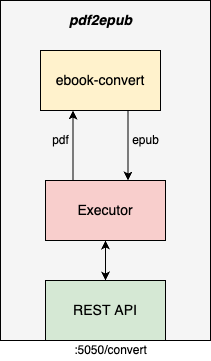
\includegraphics[width=0.25\textwidth]{img/tesi-4-pdf2epub.drawio.png}
\caption{Architettura Servizio pdf2epub}
\end{figure}
\begin{figure}[H]
\centering
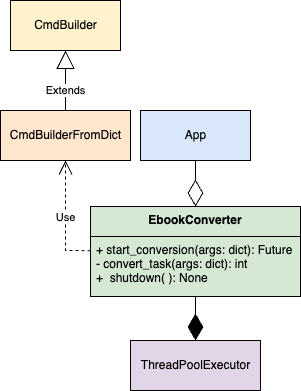
\includegraphics[width=0.6\textwidth]{img/tesi-5-pdf2epub.drawio.png}
\caption{Diagramma delle classi: pdf2epub}
\end{figure}

\subsection{Delivery pdf2epub}
La modalità di delivery scelta per il servizio \textit{pdf2epub} è tramite immagine Docker rilasciata sul container registry aziendale \textit{psacr}, per il quale si fa uso dei servizi cloud forniti da Azure\footnote{\url{https://azure.microsoft.com/en-us/services/container-registry/\#overview}}.\\
La regola che attiva la pipeline di rilascio è definita sul push di un tag sul branch principale (\textit{main}). In questo caso vengono caricate sul container registry due nuove immagini: ($i$) una con il tag esplicito che si aggiunge alle altre già caricate e ($ii$) un'altra con il tag \textit{latest}, la quale sovrascrive l'ultima immagine \textit{latest} mantenedola aggiornata all'ultima versione.
\begin{figure}[H]
\centering
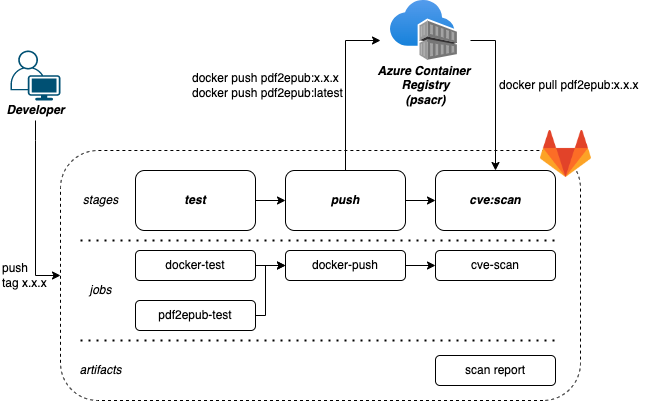
\includegraphics[width=0.9\textwidth]{img/tesi-6-pdf2html.drawio.png}
\caption{Continuous Integration/Delivery pdf2epub}
\end{figure}
\subsection{Deployment pdf2epub}
Entrambe le tipologie di documenti da convertire vengono fornite dal \textit{Sistema Redazionale}\footnote{\url{https://sisred.maggiolicloud.it}}, un applicativo mantenuto dal team Ricerca e Sviluppo del gruppo Maggioli S.p.A. il cui scopo è quello di semplificare le modalità di fruizione di tutti i contenuti editoriali (libri, riviste, contenuti web, eccetera) da parte di un insieme di servizi come motori di ricerca avanzati, applicazioni per professionisti, portali web specializzati ed applicazioni mobile. Il \textit{Sistema Redazionale} ha due obiettivi principali: ($i$) fornire supporto ai creatori di contenuto (redattori) e ($ii$) essere il mezzo che veicola questi contenuti verso l’utente finale\cite{amslaurea23043}.\\
La scelta più adeguata per il deployment del servizio \textit{pdf2epub} è il suo inserimento tra i microservizi che compongono il \textit{Sistema Redazionale} (in modo analogo al microservizio \textit{pdf2html} già presente). I principali vantaggi di questa scelta sono:
\begin{itemize}
    \item Presenza di un \textit{Application Gateway} che si occupa di autenticare le richieste e reindirizzarle verso il microservizio corretto. Non è necessario quindi esporre direttamente \textit{pdf2epub} e non è necessario gestire l'autenticazione degli utenti.
    \item Gestione/archiviazione delle conversioni rimandata al backend. Il backend si occupa di convertire in modo asincrono i documenti già memorizzati in formato pdf oppure quando ne vengono caricati di nuovi. In questo modo si ottimizza l'intero sistema effettuando tendenzialmente una unica conversione per documento piuttosto che ad ogni richiesta da parte degli utenti finali.
\end{itemize}
\begin{figure}[H]
\centering
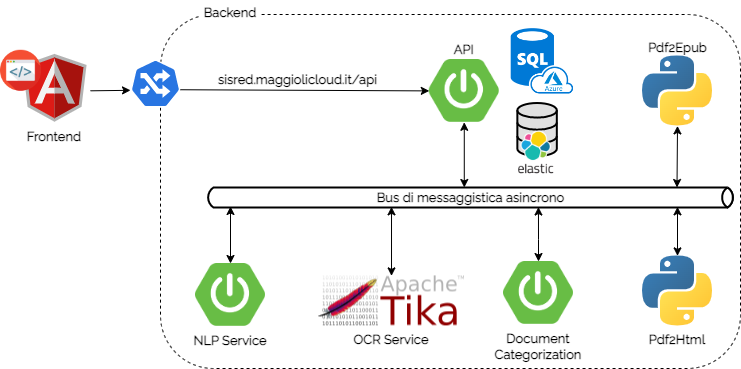
\includegraphics[width=1\textwidth]{img/tesi-7-sisred.drawio.png}
\caption{Architettura Aggiornata del Sistema Redazionale}
\end{figure}

\chapter{Capitolo}
\label{ch:capitolo3}
% !TeX root = ../main.tex

% descrivere in questo capitolo il processo tipico di sviluppo delle applicazioni mobile (android e ios) in modo da determinare le fasi automatizzabili per la definizione della CICD (da descrivere nel capitolo successivo)
% quali parti del processo sono in comune? quali tool servono? 

\end{document}
